% Chapter 10: Synthetic Data Generation
\section{Synthetic Health Data Generation Pipeline}

\subsection{Data Challenge}
Collecting labeled health training data from real wearables is expensive, time-consuming, and privacy-constrained. Anomalies are rare (a healthy user may never experience tachycardia), and annotation requires medical expertise. Synthetic generation provides large-volume, fully-labeled data covering all scenarios.

\subsection{Physiological Models}
Each activity state has characteristic vital sign distributions:

\begin{table}[H]
\centering
\caption{Activity-Specific Physiological Parameters}
\label{tab:physio}
\begin{tabular}{lcccc}
\toprule
\textbf{Activity} & \textbf{HR ($\mu \pm \sigma$)} & \textbf{Steps/hr} & \textbf{Cal/hr} & \textbf{Dist} \\
\midrule
Sleep & $55 \pm 5$ & 0 & $50 \pm 10$ & 0 \\
Rest & $70 \pm 8$ & $100 \pm 50$ & $80 \pm 15$ & 0.1 \\
Walk & $95 \pm 10$ & $3500 \pm 500$ & $200 \pm 30$ & 3.5 \\
Run & $140 \pm 15$ & $8000 \pm 1000$ & $500 \pm 80$ & 8.0 \\
Exercise & $130 \pm 12$ & $5000 \pm 800$ & $400 \pm 60$ & 4.0 \\
Other & $75 \pm 12$ & $200 \pm 150$ & $100 \pm 25$ & 0.2 \\
\bottomrule
\end{tabular}
\end{table}

Heart rate generation: $HR = \mu_{activity} + \sigma_{activity} \cdot \mathcal{N}(0, 1) + \epsilon_{noise}$, where $\epsilon_{noise} \sim \text{Uniform}(-3, 3)$.

\subsection{Context-Aware Anomaly Injection}
The critical insight: identical vital sign values receive different labels based on activity context. HR of 150 during exercise is normal; HR of 150 at rest is anomalous.

\begin{table}[H]
\centering
\caption{Anomaly Scenario Definitions}
\label{tab:scenarios}
\begin{tabular}{llcc}
\toprule
\textbf{Scenario} & \textbf{HR Range} & \textbf{Context} & \textbf{Label} \\
\midrule
Tachycardia & 150--180 BPM & At rest & Anomaly \\
Bradycardia & 30--45 BPM & At rest & Anomaly \\
Exercise HR & 130--160 BPM & Exercising & Normal \\
Sleep HR & 45--55 BPM & Sleeping & Normal \\
\bottomrule
\end{tabular}
\end{table}

\subsection{Dataset Composition}

\begin{figure}[H]
\centering
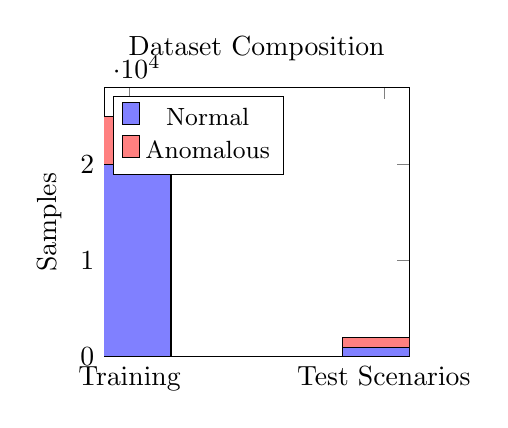
\begin{tikzpicture}
\begin{axis}[
    ybar stacked, bar width=30pt, ylabel={Samples},
    symbolic x coords={Training, Test Scenarios},
    xtick=data, ymin=0, ymax=28000,
    legend pos=north west, legend style={font=\small},
    width=0.45\textwidth, height=5cm,
    title={Dataset Composition},
]
\addplot[fill=blue!50] coordinates {(Training, 20000) (Test Scenarios, 1000)};
\addlegendentry{Normal}
\addplot[fill=red!50] coordinates {(Training, 5000) (Test Scenarios, 1000)};
\addlegendentry{Anomalous}
\end{axis}
\end{tikzpicture}
\caption{Normal vs anomalous sample distribution.}
\label{fig:dataset}
\end{figure}

\subsection{Validation Against Medical Ranges}
All synthetic parameters validate against published medical reference ranges: resting HR 60--100 BPM ($\mu$=70.2), sleep HR 40--60 BPM ($\mu$=55.1), exercise HR 100--170 BPM ($\mu$=135.4), daily steps 5K--10K ($\mu$=6,840).

\subsection{Model Performance on Synthetic Data}
Models trained on synthetic data achieve: GradientBoosting F1=0.995, XGBoost accuracy=85.8\%. Scenario test results: normal rest 99.8\% correct, normal exercise 99.6\%, tachycardia detection 99.4\%, bradycardia detection 99.2\%, exercise spike (no false alarm) 98.8\%.

\subsection{Scatter Plot: Normal vs Anomalous}

\begin{figure}[H]
\centering
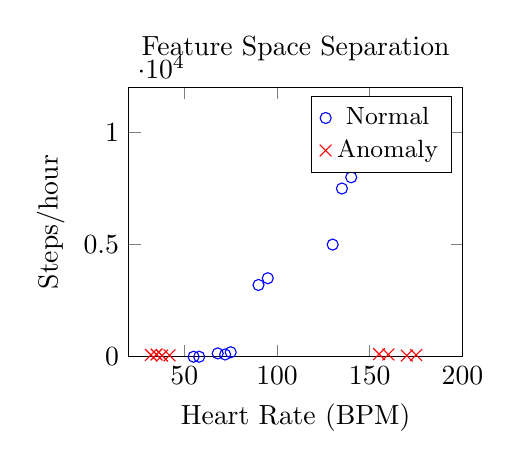
\begin{tikzpicture}
\begin{axis}[
    xlabel={Heart Rate (BPM)}, ylabel={Steps/hour},
    xmin=20, xmax=200, ymin=0, ymax=12000,
    legend pos=north east, legend style={font=\small},
    width=0.48\textwidth, height=5cm,
    title={Feature Space Separation},
]
\addplot[only marks, mark=o, blue, mark size=2pt] coordinates {
    (72, 100) (68, 150) (75, 200) (95, 3500) (90, 3200)
    (140, 8000) (135, 7500) (130, 5000) (55, 0) (58, 0)
};
\addlegendentry{Normal}
\addplot[only marks, mark=x, red, mark size=3pt] coordinates {
    (160, 100) (170, 50) (175, 80) (155, 120)
    (35, 100) (38, 50) (32, 80) (42, 60)
};
\addlegendentry{Anomaly}
\end{axis}
\end{tikzpicture}
\caption{Anomalies cluster in high-HR/low-activity and low-HR/low-activity regions.}
\label{fig:scatter}
\end{figure}

\subsection{Transition to Real-World Data}
Staged approach: Phase 1 (current)---train on synthetic data. Phase 2---collect real data from pilot users (10--20). Phase 3---fine-tune on mixed data. Phase 4---train primarily on real data, synthetic for augmentation.
